\chapter{Vols de prova de fotogrametria}
\label{chap:vols-prova}

Aquest capítol presenta els dos vols de fotogrametria fets amb el sistema complet un cop estabilitzats el control i el GPS (\cref{chap:proves-vol}): el vol de prova 5, a 30~m sobre un parc, i el vol de prova 6, a 50~m sobre un camp. Tots dos han recorregut la cadena sencera --~planificació, vol automàtic amb RTK, geoetiquetat, processat i exportació~-- i serveixen per quantificar-ne el comportament, en particular el retard de l'obturador (\cref{sec:retard-obturador}).

\section{Cadena de processament}
\label{sec:cadena-processat}

\subsection{Captura}

La missió és un \emph{grid} en mode Auto a 5~m/s amb el dispar per distància. El MAP2 dispara la càmera per PWM i el SYNC2, a la sabata, retorna l'instant real de l'exposició al controlador, que el registra com a missatge \texttt{CAM} al \emph{log} (l'ordre de dispar queda registrada com a \texttt{TRIG}). La posició de cada missatge és la de l'EKF3, amb RTK Fixed i \emph{yaw} GNSS.

\subsection{Post-procés de les fotografies}
\label{sec:processament-fotos}

Les fotografies de la càmera no es poden processar tal com surten:
\begin{itemize}
    \item \textbf{Orientació.} L'etiqueta EXIF d'orientació de la Sony $\alpha$6000 depèn del rumb (la càmera apunta a nadir), mentre que els píxels són sempre de 6000~$\times$~4000. Es normalitza a \emph{Orientation}=1 en una còpia: només canvia l'etiqueta, els píxels no es toquen.
    \item \textbf{Òptica.} L'objectiu manual no grava distància focal, model ni diafragma: es reescriuen (TTArtisan 25~mm, equivalent a 38~mm, f/5,6).
    \item \textbf{Posició.} Cada fotografia s'aparella amb el seu missatge de \emph{log} (\texttt{CAM} o \texttt{TRIG}), s'hi escriuen les etiquetes GPS i es genera un fitxer de geoetiquetes amb la precisió per foto: 0,5~m en vol recte, 1,5~m als girs i 0,3~m en vertical.
    \item \textbf{Rellotge.} El rellotge de la càmera va desfasat unes 9~h respecte a UTC: l'aparellament es fa per ordre (vol 5) o per instant (vol 6), no per l'hora de l'EXIF.
\end{itemize}

Els \emph{scripts} que fan aquests passos, els \emph{logs} de vol, les fotografies corregides, els fitxers de geoetiquetes i els resultats de cada processat s'arxiven amb sumes de verificació SHA-256, de manera que cada resultat es pot regenerar des de les dades d'origen.

\subsection{Reconstrucció}

La reconstrucció es fa amb ODX 3.8.3 (\cref{sec:processament}). Es generen ortofoto, DSM, núvol de punts i models texturats en EPSG:32631.

\section{Vol de prova 5 -- parc (8 d'octubre de 2026)}
\label{sec:vol5}

\subsection{Equip i vol}

\begin{table}[H]
    \centering
    \caption{Equip i paràmetres del vol de prova 5}
    \label{tab:vol5-equip}
    \small
    \begin{tabular}{lP{9.6cm}}
        \toprule
        Concepte & Valor \\
        \midrule
        Controlador & ArduCopter 4.6.3, Kakute H7, RC CRSF, ESC DShot300 \\
        Càmera / òptica & Sony $\alpha$6000 + TTArtisan 25~mm f/2, enfocament i diafragma manuals; 1/1600~s, f/5,6 \\
        Navegació & RTK Fixed durant el 100~\% del vol als dos receptors (GPS[0] i GPS[1]), amb correccions de la base RTK pròpia \\
        Grid & 8 passades separades 6,5~m, 7,1~m entre fotos (dispar per distància), $\sim$30~m sobre el punt d'enlairament, $\sim$5~m/s \\
        Fotografies & 118, entre les 12:26 i les 12:30 (hora local) \\
        Solapament calculat & 75--77~\% frontal, 65--69~\% lateral; $\sim$11 imatges per punt \\
        Càmera respecte al dron & Girada 90$^{\circ}$ (costat llarg en el sentit de vol) \\
        \emph{Feedback} de la sabata & No disponible en aquest vol (cablejat invertit, corregit i verificat després al banc) \\
        \bottomrule
    \end{tabular}
\end{table}

\subsection{Resultats}

Es van fer dos processats amb les mateixes 118 fotografies: el primer amb les posicions GPS tal com surten del \emph{log} i el segon amb les posicions corregides pel retard de l'obturador (\cref{sec:retard-obturador}). La geometria del model és la mateixa; canvia la georeferenciació.

\begin{table}[H]
    \centering
    \caption{Resultats del processat del vol de prova 5}
    \label{tab:vol5-resultats}
    \small
    \begin{tabular}{lcc}
        \toprule
        & Sense correcció & Amb correcció del retard \\
        \midrule
        Fotos reconstruïdes & 118 de 118 & 118 de 118 \\
        Error de reprojecció & 0,90~px & 0,90~px \\
        Punts del model dispers & 173.084 & 173.401 \\
        Focal efectiva (calibrada) & 25,72~mm & 25,74~mm \\
        GSD mitjà & 0,451~cm/px & 0,452~cm/px \\
        Àrea reconstruïda & 6.633~m\textsuperscript{2} & 6.714~m\textsuperscript{2} \\
        Núvol de punts dens & 38.547.923 & 38.727.582 \\
        Diferència model--GPS, E / N / vert.\ (desv.\ est.) & 1,30 / 0,37 / 0,12~m & \textbf{0,40 / 0,14 / 0,11~m} \\
        CE90 / LE90 model--GPS & 1,80 / 0,19~m & \textbf{0,59 / 0,18~m} \\
        Temps de processat & 43~min 24~s & 41~min 34~s \\
        \bottomrule
    \end{tabular}
\end{table}

Els errors model--GPS comparen el model amb les posicions de les fotos: mesuren la coherència interna, \textbf{no la precisió absoluta}, que requereix punts de comprovació independents (\cref{sec:gcp}). La correcció del retard redueix la diferència horitzontal de l'ordre d'1,3~m a $\sim$0,4~m, i les posicions de càmera georeferenciades es mouen com a màxim 0,31~m entre els dos processats, amb una rotació del model de $0{,}2^{\circ}$.

\begin{figure}[H]
    \centering
    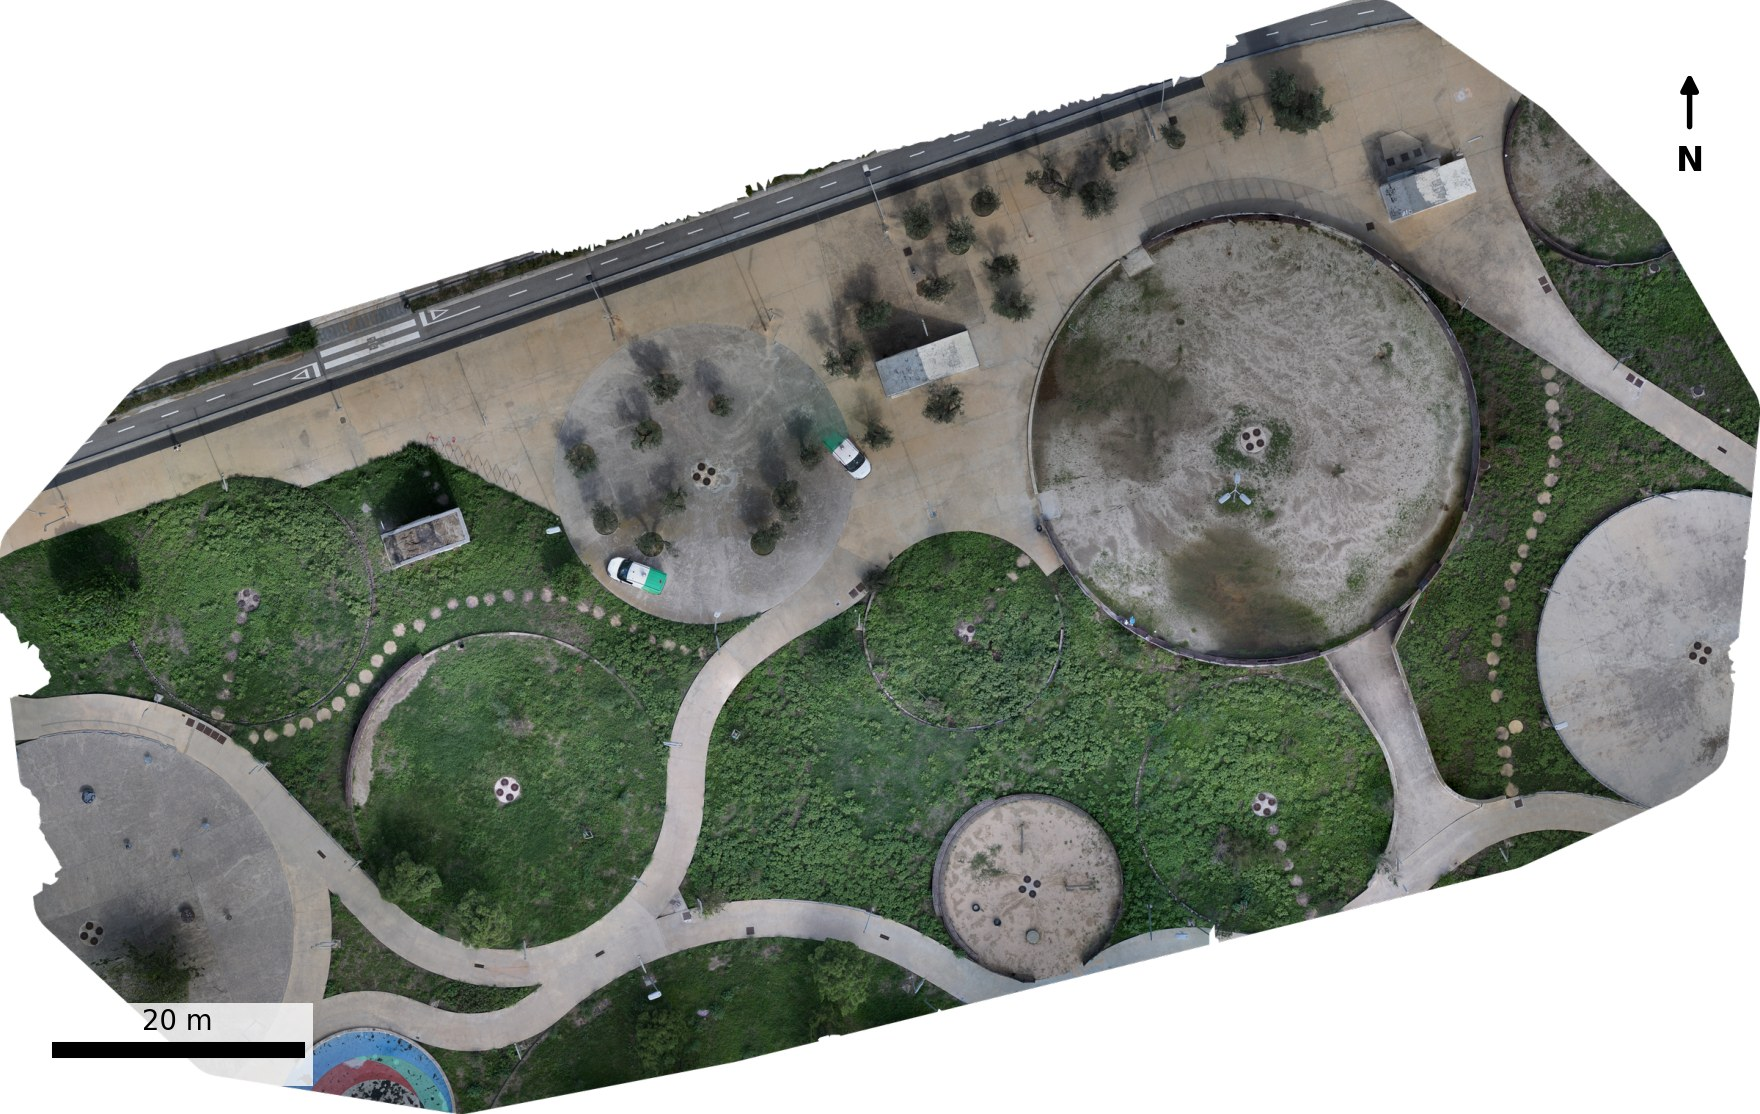
\includegraphics[width=\textwidth]{img/vol5_ortofoto.jpg}
    \caption{Ortofoto del vol de prova 5 (1~cm/px, EPSG:32631), processat amb posicions corregides pel retard de l'obturador.}
    \label{fig:vol5-ortofoto}
\end{figure}

L'ortofoto (14.084~$\times$~8.918~px a 1~cm/px) és coherent: sense costures ni deformació en forma de bol, amb vials i rotondes coherents i nítida a escala 1:1 (juntes de formigó, fulles individuals). El DSM (7.041~$\times$~4.458~px a 2~cm/px) és net a l'interior (edificis plans, arbres com a relleu); la primera i l'última passada i els extrems mostren estries per haver-hi poques vistes, de manera que convé retallar el DSM al polígon d'interès o ampliar el pla de vol un \emph{footprint} més enllà de la zona.

\begin{figure}[H]
    \centering
    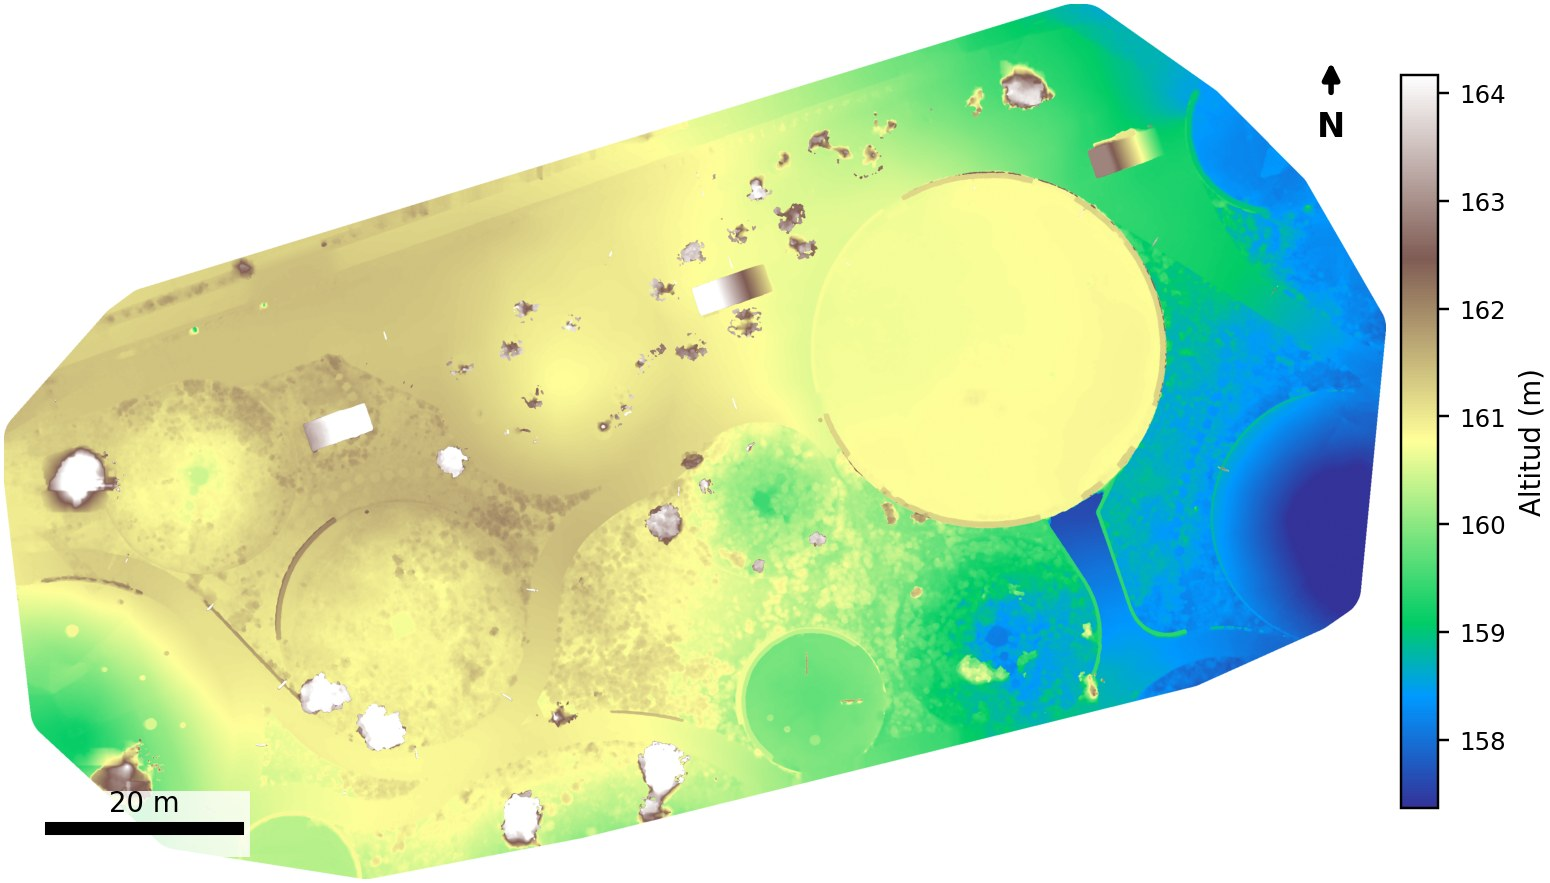
\includegraphics[width=\textwidth]{img/vol5_dsm.jpg}
    \caption{Model digital de superfície del vol de prova 5 (2~cm/px). Els buits blancs són copes d'arbres per sobre del rang de la paleta.}
    \label{fig:vol5-dsm}
\end{figure}

\section{Vol de prova 6 -- camp (13 d'octubre de 2026)}
\label{sec:vol6}

\subsection{Equip i vols}

El vol de prova 6 consta de dos vols a $\sim$50~m (àrea de $\sim$180~$\times$~150~m) amb el mateix dron i càmera que el 5 i amb els paràmetres de bateria ja calibrats. S'hi va validar el \emph{feedback} de la sabata (\texttt{CAM}) i la planificació a 50~m. Es van fer a l'alba, amb el sol entre $-3^{\circ}$ i $+1^{\circ}$ sobre l'horitzó, de manera que les fotografies van sortir molt fosques.

\begin{table}[H]
    \centering
    \caption{Registre dels dos vols del vol de prova 6}
    \label{tab:vol6-logs}
    \small
    \begin{tabular}{lcc}
        \toprule
        & Vol 1 (07:46) & Vol 2 (07:57) \\
        \midrule
        mAh consumits (\texttt{CurrTot} / integral) & 2.326 / 2.306 & 2.434 / 2.426 \\
        Motors en marxa & 5,5~min & 11,3~min (dos armats) \\
        Tensió inicial / mínima / final & 24,65 / 21,25 / 21,95~V & 24,73 / 21,13 / 21,95~V \\
        Corrent mitjà / màxim & 25 / 56~A & 22 / 58~A \\
        \emph{Failsafe} de bateria baixa & 268~s, 21,52~V, 1.887~mAh & 635~s, 21,48~V, 2.012~mAh \\
        Dispars \texttt{TRIG} / \texttt{CAM} / fotos & 94 / 93 / 94 & 110 / 110 / 110 \\
        \bottomrule
    \end{tabular}
\end{table}

\begin{itemize}
    \item \textbf{Bateria.} Els dos vols acaben per \emph{failsafe} de bateria baixa quan només s'ha gastat el 47--50~\% dels 4.000~mAh: la tensió instantània cau per sota de 21,6~V sota càrrega (\texttt{BATT\_FS\_VOLTSRC=0}). Cal comparar els mAh amb el que torna el carregador.
    \item \textbf{Exposició.} 1/1600~s, f/5,6, ISO 1600 (sostre de l'ISO automàtic): les fotografies queden unes 6~\emph{stops} subexposades, i la llum de l'escena és de 8,5--11,9~\emph{stops} per sota de la del vol 5 (sol a 40$^{\circ}$). El marge màxim de la càmera és de 5,7~\emph{stops}. No és cap avaria: és una limitació de llum.
    \item \textbf{Feedback.} Amb \texttt{TRIG}, \texttt{CAM} i fotografies en proporció 1:1 (110 de 110 al vol 2), l'aparellament es fa per instant. Hi ha una foto manual sense \texttt{TRIG} i un \texttt{TRIG} sense foto.
\end{itemize}

\pendent{Repetir aquest vol amb el sol a més de 10--15$^{\circ}$, que és la condició que el fa aprofitable (el lot actual només serveix de prova).}

\subsection{Processat del vol 2}

El vol 1 no és aprofitable (el guany digital $\times 551$ no recupera senyal: 2 coincidències entre fotos consecutives, igual que el soroll). Del vol 2 es van processar les 110 fotografies amb un guany lineal de $\times 2$ a $\times 97$ (mediana $\times 49$); \textbf{la geometria és vàlida, però els colors i els valors radiomètrics no ho són} (to verd-blavós, soroll alt), per la qual cosa aquest lot no serveix per a color ni índexs de vegetació.

\begin{table}[H]
    \centering
    \caption{Resultats del processat del vol 2 del vol de prova 6}
    \label{tab:vol6-resultats}
    \begin{tabular}{ll}
        \toprule
        Concepte & Valor \\
        \midrule
        Fotos reconstruïdes & 110 de 110 (1 component) \\
        Punts del model dispers / observacions & 101.094 / 354.361 \\
        Error de reprojecció & 1,82~px \\
        GSD mitjà / àrea reconstruïda & 0,743~cm/px / 30.626~m\textsuperscript{2} \\
        Núvol de punts dens & 27.207.845 punts \\
        Calibració de la càmera & focal 25,79~mm \\
        Diferència model--GPS (E / N / vert.) & 0,30 / 0,32 / 0,30~m; CE90 0,57~m, LE90 0,27~m \\
        Resolució d'ortofoto / DSM & 3~cm/px / 5~cm/px \\
        Temps de processat & 29~min 42~s \\
        \bottomrule
    \end{tabular}
\end{table}

La qualitat és inferior a la del vol 5 (reprojecció de 1,82~px davant de 0,90~px): és coherent amb el soroll de les imatges, que fa preferir una resolució de treball més gran (3~cm/px). L'ortofoto (7.799~$\times$~7.071~px) mostra el camp, els camins, la corba del camí i un vehicle blanc reconeixibles, amb to verd-blavós i soroll visibles i un contorn oest irregular. El DSM (4.679~$\times$~4.242~px) és detallat a l'interior (solcs, rodades) i té estries i una quadrícula d'interpolació a la vora oest i nord-oest.

\begin{figure}[H]
    \centering
    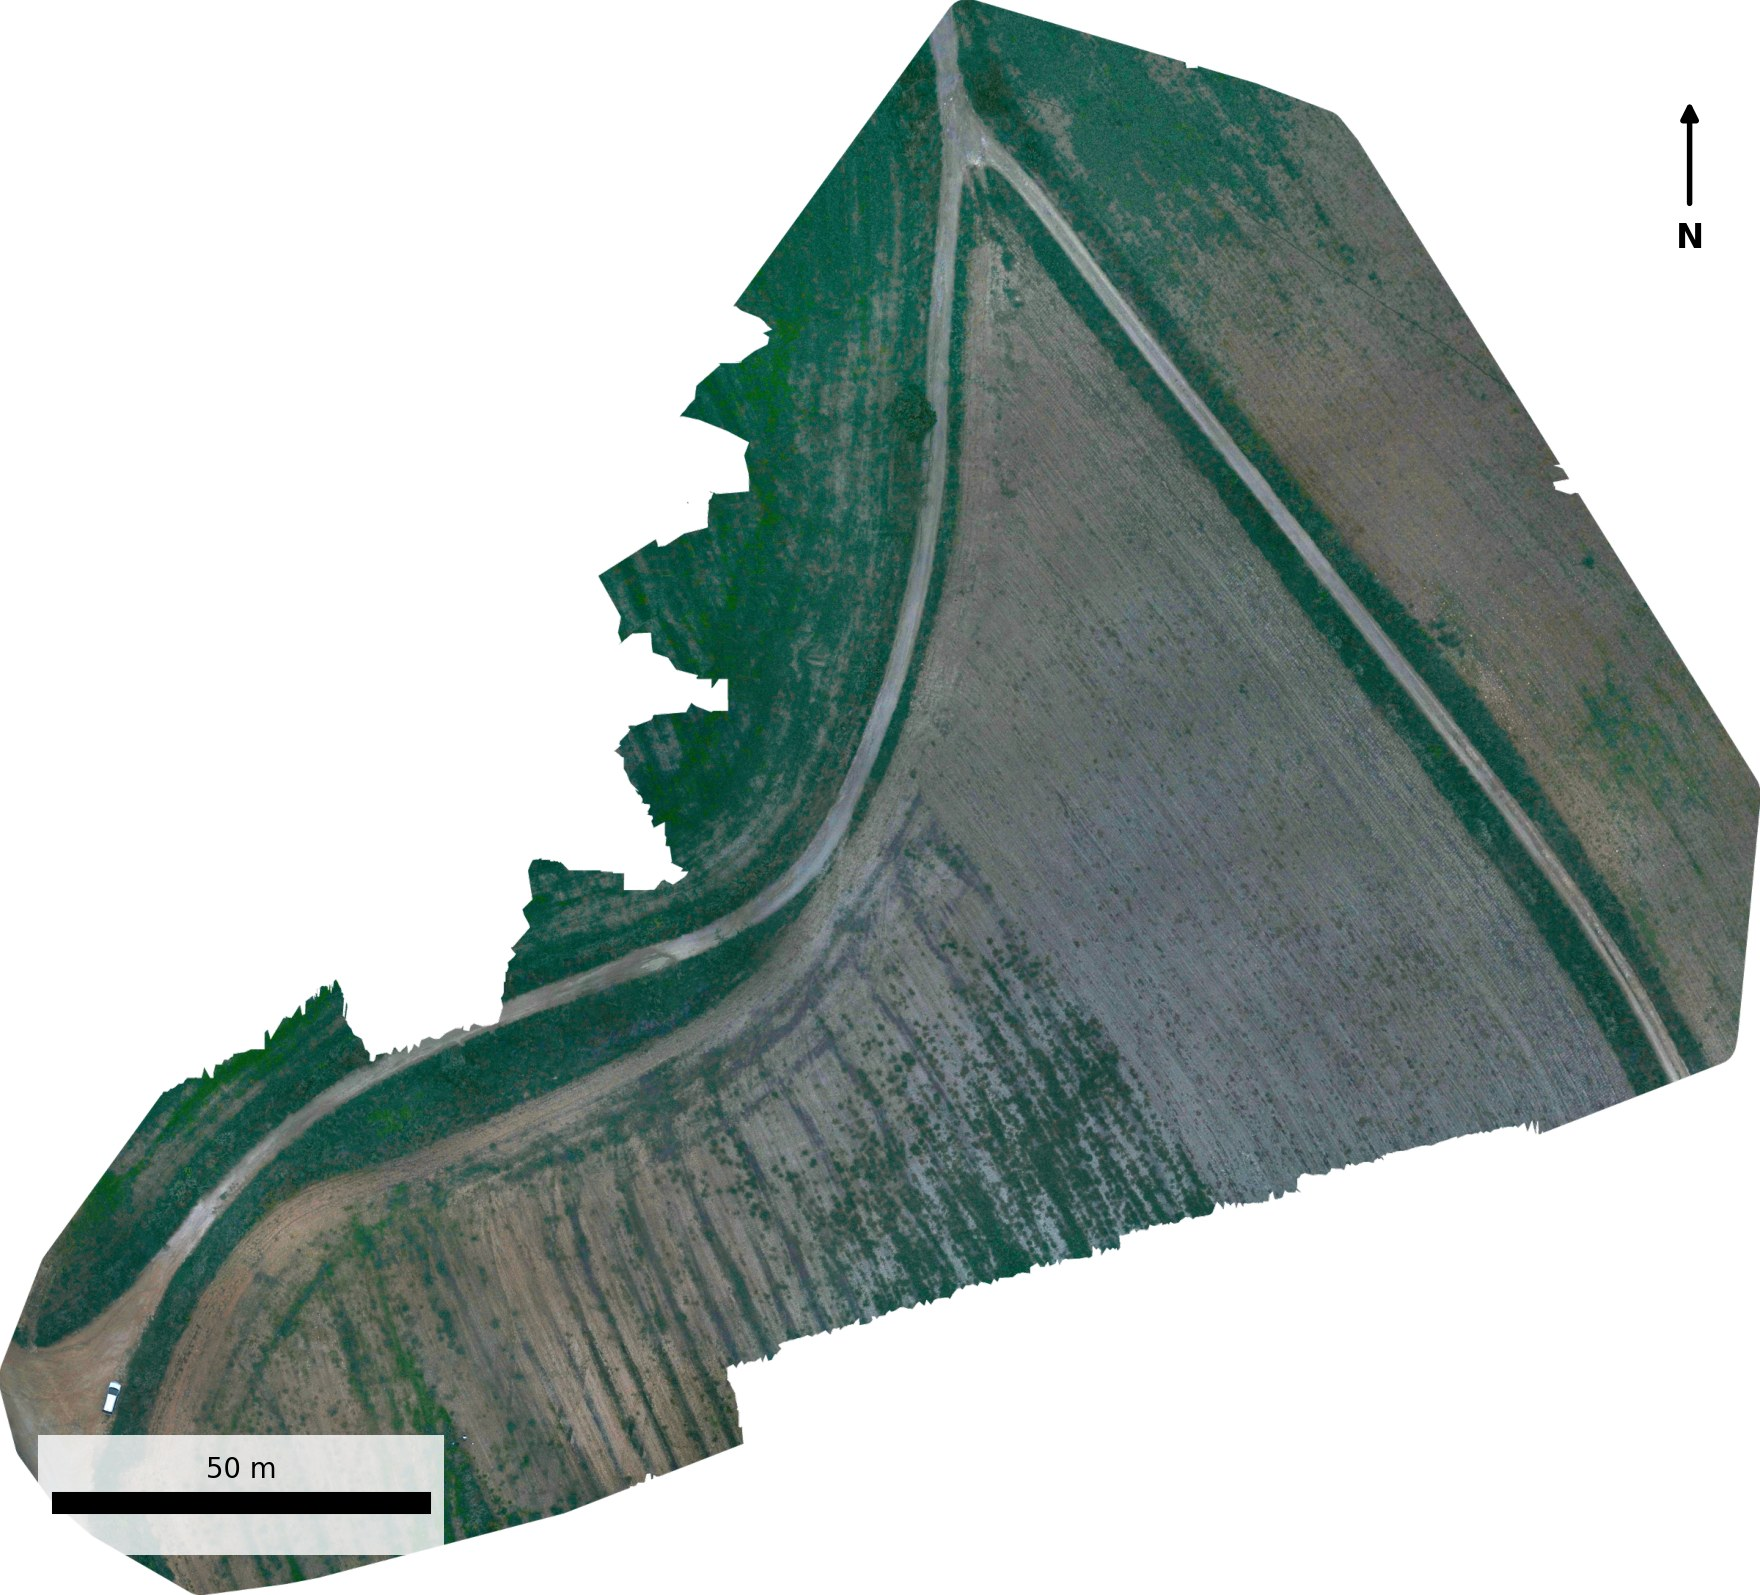
\includegraphics[width=0.85\textwidth]{img/vol6_ortofoto.jpg}
    \caption{Ortofoto del vol 2 de la prova 6 (3~cm/px). Les imatges s'han realçat digitalment: només la geometria és vàlida, no el color.}
    \label{fig:vol6-ortofoto}
\end{figure}

\begin{figure}[H]
    \centering
    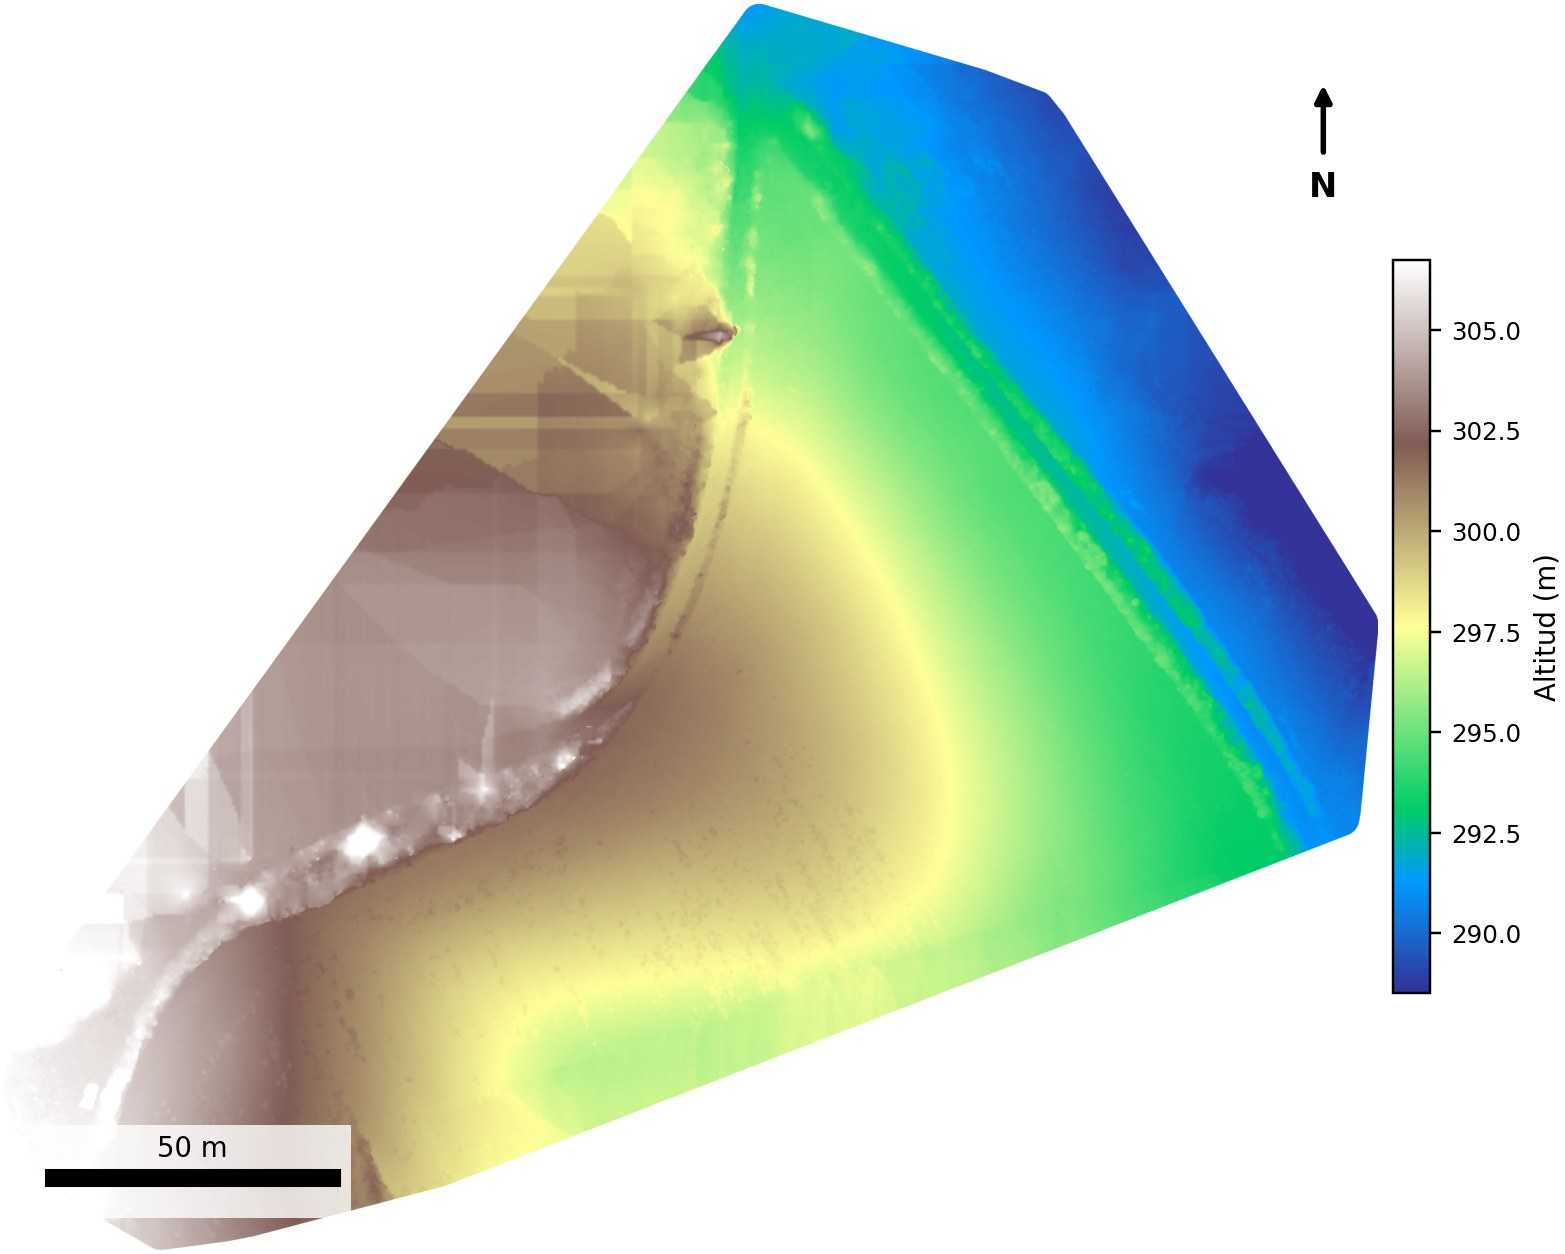
\includegraphics[width=0.85\textwidth]{img/vol6_dsm.jpg}
    \caption{Model digital de superfície del vol 2 de la prova 6 (5~cm/px).}
    \label{fig:vol6-dsm}
\end{figure}

\section{Retard de l'obturador}
\label{sec:retard-obturador}

L'ordre de dispar del controlador i l'exposició real no coincideixen: entre ells hi ha el retard del MAP2, de la càmera i, possiblement, el de la posició GPS/EKF. Com que el dron es mou a $\sim$5~m/s, un retard de 0,27~s equival a $\sim$1,3~m de desplaçament, molt per sobre de la precisió centimètrica buscada.

\subsection{Mètode}

Per a cada foto es compara la posició GPS del \emph{log} amb la posició de càmera reconstruïda pel model fotogramètric. Si el retard és $\tau$, el residu GPS $-$ model val $-v\tau$: té signe oposat a les passades d'anada i de tornada i un desplaçament global proper a zero, cosa que el distingeix d'un error sistemàtic de georeferenciació.

\subsection{Resultats}

\begin{table}[H]
    \centering
    \caption{Estimacions del retard de l'obturador}
    \label{tab:retard}
    \small
    \begin{tabular}{P{5.2cm}P{4.2cm}P{4.6cm}}
        \toprule
        Mesura & Retard & Observacions \\
        \midrule
        Vol 5, posicions \texttt{TRIG} & $\tau = 0{,}268 \pm 0{,}009$~s & ENE 0,277~$\pm$~0,007; WSW 0,267~$\pm$~0,014 \\
        Vol 5 amb posicions corregides & residual $0{,}004 \pm 0{,}007$~s & Residu horitzontal mediana 1,38~m $\rightarrow$ 0,35--0,49~m \\
        Vol 6, \texttt{TRIG}$\rightarrow$\texttt{CAM} & mediana 0,34~s (0,11--0,40) & Mesurat directament al \emph{log} \\
        Vol 6, posicions \texttt{CAM} & residual $-0{,}056 \pm 0{,}011$~s & La posició \texttt{CAM} va $\sim$56~ms per davant de l'exposició \\
        Vol 6, \texttt{TRIG}$\rightarrow$exposició & $0{,}34 - 0{,}056 \approx 0{,}28$~s & D'acord amb el vol 5 per un camí independent \\
        Banc, comandament$\rightarrow$obturador & 0,12--0,19~s & No explica tot el retard en vol \\
        \bottomrule
    \end{tabular}
\end{table}

Dos mètodes independents --~el residu fotogramètric del vol 5 i la combinació de \texttt{TRIG}, \texttt{CAM} i residu del vol 6~-- coincideixen en 0,27--0,28~s. És un retard \emph{efectiu}: suma el de l'obturador i, possiblement, el de la posició GPS/EKF, i un desplaçament fix de l'antena respecte a la càmera cap endavant es confon amb ell (si es deixa com a incògnita, el retard surt 0,34~$\pm$~0,03~s i el desplaçament 0,32~$\pm$~0,16~m, i no es poden separar). El retard del banc no explica tot el valor en vol; no es pot separar sense \emph{feedback}.

\subsection{Conseqüències per al geoetiquetat}

Amb \emph{feedback} (\texttt{CAM}), la posició és la de l'exposició real i només queda un retard residual de $-0{,}056$~s ($\sim$0,3~m a 5~m/s), que es pot compensar. Sense \emph{feedback} cal desplaçar la posició $v\cdot\tau$ amb $\tau \approx 0{,}27$~s i precisions per foto més amples. Aquest és el motiu pel qual el \emph{feedback} de la sabata és obligatori per a precisió centimètrica (\cref{sec:decisions}).

\section{Balanç dels vols de prova}
\label{sec:balanc-vols}

\textbf{Què ha funcionat.}
\begin{itemize}
    \item La cadena completa, de la planificació al DSM, amb RTK Fixed durant tot el vol als dos receptors i \emph{yaw} GNSS vàlid.
    \item Una geometria de qualitat fotogramètrica: reprojecció de 0,90~px, 118 de 118 fotos reconstruïdes i un GSD (0,451~cm/px) coherent amb l'alçada de vol i la focal calibrada (\cref{sec:planificacio-vol}).
    \item El \emph{feedback} de la sabata (110 de 110 al vol 6) i la quantificació independent del retard de l'obturador.
\end{itemize}

\textbf{Limitacions.}
\begin{itemize}
    \item No hi ha punts de control ni de comprovació: no es pot afirmar una precisió absoluta. Les xifres model--GPS són de coherència interna.
    \item La posició absoluta depèn de la base RTK, que en aquests vols va fer un \emph{survey-in} a cada sessió amb l'antena a 122~cm (\cref{subsec:muntatge-base}). No es va registrar la posició resultant, i l'error absolut és de l'ordre de metres, comú a tot el vol.
    \item Del vol 5 no es disposa de les condicions meteorològiques, la massa en vol ni la bateria utilitzada: el \emph{log} i les fotografies són l'únic registre.
    \item La llum limita l'operació: cal volar amb el sol a més de 10--15$^{\circ}$ (o, amb poca llum, 1/800~s, f/4 i ISO 3200 al límit).
    \item L'autonomia és curta: els \emph{failsafes} de bateria baixa actuen a mig consum per la caiguda de tensió sota càrrega (\cref{sec:autonomia}).
    \item El DSM presenta estries a la perifèria: cal ampliar el pla de vol un \emph{footprint} més enllà de la zona d'interès.
\end{itemize}

\textbf{Pròxims passos.} Repetir el vol de camp amb el sol alt, mesurar punts de control i de comprovació a terra per establir la precisió absoluta, reestimar el retard amb \emph{feedback} i millorar l'autonomia (\cref{sec:propulsor}). La llista completa de tasques pendents és a \cref{sec:pendents-proves-vol}.

\pendent{La precisió absoluta (horitzontal i vertical) del producte final continua sense mesurar: tots els errors d'aquest capítol són de coherència interna.}
